%! Author = spruhs
%! Date = 25.02.25

% Preamble
\documentclass[11pt]{article}

% Packages
\usepackage[utf8]{inputenc}
\usepackage[T1]{fontenc}
\usepackage[ngerman]{babel}
\usepackage{graphicx}
\usepackage{tocloft}
\usepackage{appendix}
\usepackage{csquotes}
\usepackage[
    backend=biber,
    style=alphabetic,
]{biblatex}
\addbibresource{literaturverzeichnis.bib}

% Document
\begin{document}

    \begin{titlepage}
        \centering
        {\scshape\LARGE Seminar 1908 Moderne Programmiertechniken und -Methoden -Sommer 2025 \par}
        \vspace{1cm}
        {\huge\bfseries Kotlin statt Java\par}
        \vspace{1.5cm}
        {\scshape\Large Fabian Spruhs\par}
        {\scshape fabian@spruhs.com\par}
        \vspace{2cm}
        {\Large\itshape Studiengang Bachelor Informatik\par}
        \vspace{2cm}


        {\large \today\par}
    \end{titlepage}

    \tableofcontents
    \newpage

    \section{bla bla}
        java
    \subsection{bla bla 2}
        more content

    \printbibliography[
        heading=bibintoc,
        title={Literaturverzeichnis}
    ]

    \appendix
    \section{Anhang}

    \begin{figure}[h]
        \centering
        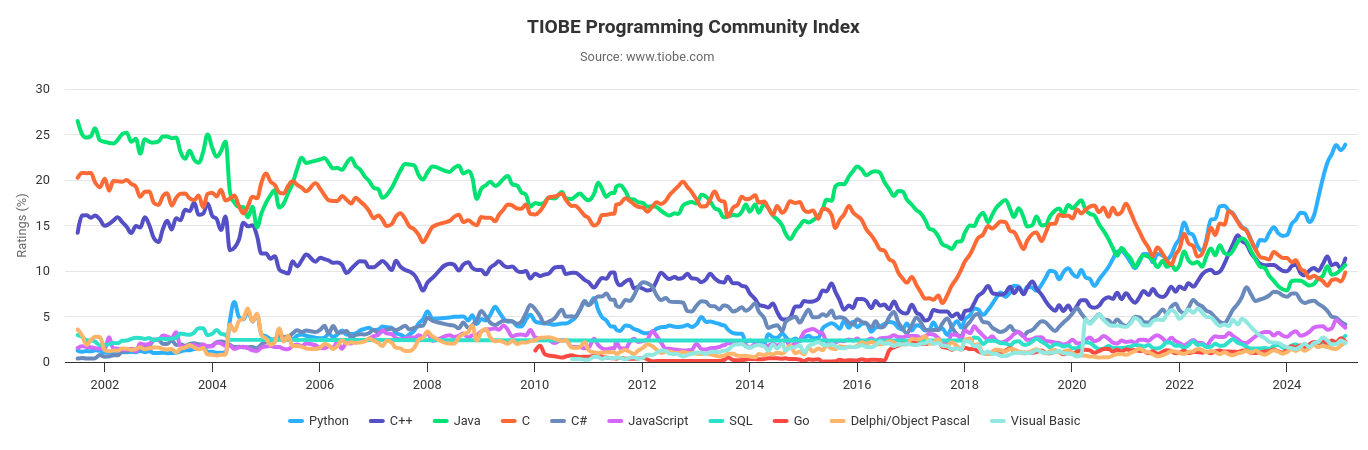
\includegraphics[width=0.8\textwidth]{pictures/Screenshot 2025-02-26 at 19-53-49 TIOBE Index - TIOBE}
        \caption{Beschreibung der ersten Grafik}
        \label{fig:grafik1}
    \end{figure}

    \begin{figure}[h]
        \centering
        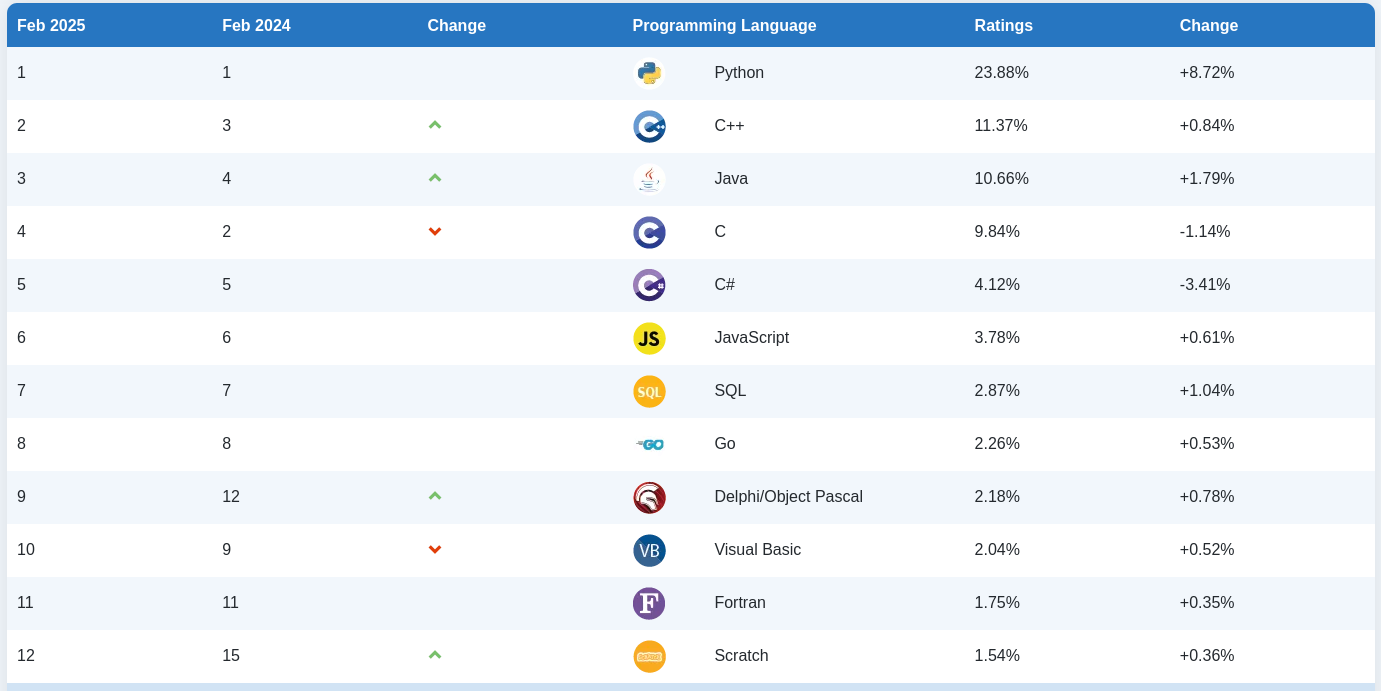
\includegraphics[width=0.8\textwidth]{pictures/Screenshot 2025-02-26 at 19-54-42 TIOBE Index - TIOBE}
        \caption{Beschreibung der ersten Grafik}
        \label{fig:grafik2}
    \end{figure}

    \cite{insel}
    \cite{kotlin-handbuch}



\end{document}